\documentclass[12pt,letterpaper,twoside]{article}
\usepackage{../cme211}
\usepackage{algorithm2e}

\def\D{\mathrm{d}}
\usepackage{atbegshi}% http://ctan.org/pkg/atbegshi

\begin{document}
\title{Lecture 12: Functions and File IO in C++, \\ Preprocessor Step of Compilation\vspace{-5ex}}
\date{Fall 2020}
\maketitle

{\footnotesize
\paragraph{Topics:} Functions, Command line arguments and
formatting, (file) IO, pre-processor and \texttt{\#include}.
}
\vspace{-3ex}

\section{Functions in C++}
Functions allow us to decompose a program into smaller components
It is easier to implement, test, and debug portions of a program in isolation;
further, decomposition allows work to be spread among many people working mostly
independently. When done properly, resulting programs are easier to understand and
maintain: we seek to eliminate duplicated code and reuse functions across 
multiple programs. 
\href{https://en.wikipedia.org/wiki/Don%27t_repeat_yourself#DRY_vs_WET_solutions}
{Don't Repeat Yourself (DRY vs. WET code)}.


\begin{cpp}
int sum(int a, int b) {
  int c = a + b;
  return c;
}
\end{cpp}

Components:

{\footnotesize
\begin{verbatim}
return_type function_name(argument_type1 argument_var1, ...) {
   // function body
   return return_var; // return_var must have return_type
}
\end{verbatim}
}

Consider \texttt{src/sum1.cpp}:.
\begin{cpp}
#include <iostream>
int sum(int a, int b) {
  int c = a + b;
  return c;
}

int main() {
  int a = 2, b = 3;
  int c = sum(a,b);
  std::cout << "c = " << c << std::endl;
}
\end{cpp}

We can compile with \texttt{g++ -Wall -Wextra -Wconversion sum1.cpp -o sum1} and run:

\begin{verbatim}
$ ./sum1
c = 5
\end{verbatim}

\subsection{Order of Declaration Matters}
Consider \texttt{src/sum2.cpp}: we attempt to \emph{use} a function \emph{before} defining it. This yields an error.

\begin{cpp}
#include <iostream>

int main() {
  int a = 2, b = 3;
  // the compiler does not yet know about sum()
  int c = sum(a,b);
  std::cout << "c = " << c << std::endl;
}

int sum(int a, int b) {
  int c = a + b;
  return c;
}
\end{cpp}

The compiler imports the objects defined in \texttt{iostream}, but when it gets
to the expression \texttt{sum(a,b)} it doesn't find an object named \texttt{sum} to be 
defined in the current scope.
Output:

{\small
\begin{verbatim}
$ g++ -Wall -Wextra -Wconversion sum2.cpp -o sum2
sum2.cpp: In function 'int main()':
sum2.cpp:7:18: error: 'sum' was not declared in this scope
  int c = sum(a,b);                 ^
\end{verbatim}
}
\paragraph{Function Declaration}
A \href{https://en.cppreference.com/w/cpp/language/function}{function \emph{declaration}} 
specifies the function name, input
argument type(s), and output type only; it 
need not specify the implementation (code) for the function, however it does
critically specify the information needed from a compiler in order to validate
its use within a program.

\paragraph{Function Definition}
A function \emph{definition} is the code that implements the function, and 
it is legal to call a function if it has been defined or
\emph{simply declared}; see \texttt{src/sum3.cpp}.

\begin{cpp}
#include <iostream>

// Forward declaration or prototype
int sum(int a, int b);

int main() {
  int a = 2, b = 3;
  int c = sum(a,b);
  std::cout << "c = " << c << std::endl;
}

// Function definition
int sum(int a, int b) {
  int c = a + b;
  return c;
}
\end{cpp}
{\small
\begin{verbatim}
$ g++ -Wall -Wextra -Wconversion sum3.cpp -o sum3
$ ./sum3
c = 5
\end{verbatim}
}

\subsection{Functions, Data Types, and Implicit Casting}
\subsubsection{Arguments (and Return Types) Cast to Match Function Declaration}
What happens if we provide arguments ``with incorrect type''? It really depends on what sub-routines the compiler finds (i.e. what we've defined and \texttt{\#include}d).\footnote{In CME 212, we'll emphasize a bit more details around
\href{https://en.cppreference.com/w/cpp/language/lookup}{lookup}, which may involve 
\href{https://en.cppreference.com/w/cpp/language/adl}{inspecting arguments via argument dependent lookup} (and possibly template argument deduction) to disambiguate overloaded functions, 
and how the compiler
determines which sub-routine to execute when a \href{https://en.cppreference.com/w/cpp/language/identifiers#Names}{\texttt{name}} is encountered.} 
Consider \texttt{src/datatypes1.cpp}.

\begin{cpp}
#include <iostream>

int sum(int a, int b) {
  return a + b;
}

int main() {
  double a = 2.7, b = 3.8;
  int c = sum(a,b);   // Oops! Our sum() only expects integer args.
  std::cout << "c = " << c << std::endl;
}
\end{cpp}

\paragraph{A sub-routine accepting numeric inputs is found, but implicit casting required}
Above, the compiler runs into \texttt{sum(a,b)} and sees that there is only a single 
\texttt{sum()} function defined. This is good news, however the function happens to require
\texttt{int}eger arguments. We learned previously that although C++ is strongly typed,
some implicit casting can occur between numeric types.
With warning flags enabled, we are told that
variables \texttt{a} and \texttt{b} are implicitly being cast to \texttt{int} such that we can
proceed with evaluating \texttt{sum(a,b)}. Output:

{\small
\begin{verbatim}
$ g++ -Wall -Wextra -Wconversion datatypes1.cpp -o datatypes1
datatypes1.cpp: In function 'int main()':
datatypes1.cpp:14:18: warning: conversion to 'int' from 'double' may alter its value [-Wconversion]
  int c = sum(a,b);
              ^
datatypes1.cpp:14:18: warning: conversion to 'int' from 'double' may alter its value [-Wconversion]
$ ./datatypes1
c = 5
\end{verbatim}
}

\paragraph{Return Value (Implicitly) Cast to Match Function Declaration}
Consider \texttt{src/datatypes2.cpp}:

\begin{cpp}
#include <iostream>
int sum(int a, int b) {
  double c = a + b;
  return c; // we are not returning the correct type
}

int main() {
  int a = 2, b = 3;
  int c = sum(a,b);
  std::cout << "c = " << c << std::endl;
}
\end{cpp}

{\small
\begin{verbatim}
$ g++ -Wall -Wextra -Wconversion datatypes2.cpp -o datatypes2
datatypes2.cpp: In function 'int sum(int, int)':
datatypes2.cpp:6:10: warning: conversion to 'int' from 'double' may alter its value [-Wconversion]
  return c;
         ^
$ ./datatypes2
c = 5
\end{verbatim}
}

\paragraph{Explicit Casting} Of course, we may explicitly instruct the compiler to obey
a cast command,
\texttt{src/datatypes3.cpp}.

\begin{cpp}
#include <iostream>

int sum(int a, int b) {
  double c = a + b;
  return (int)c;
}

int main() {
  double a = 2.7, b = 3.8;
  int c = sum((int)a,(int)b);
  std::cout << "c = " << c << std::endl;
}
\end{cpp}

Output after compiling with \texttt{g++ -Wall -Wextra -Wconversion datatypes3.cpp -o datatypes3}:

{\small
\begin{verbatim}
$ ./datatypes3
c = 5
\end{verbatim}
}

\subsection{\texttt{void} Data Type: Absent/Unspecified}
We can think of using the \texttt{void} keyword to indicate absence of data, e.g.
\texttt{src/void1.cpp}.

\begin{cpp}
#include <iostream>

void printHeader(void) {
  std::cout << "-------------------------" << std::endl;
  std::cout << "      MySolver v1.0      " << std::endl;
  std::cout << "-------------------------" << std::endl;
}

int main() {
  printHeader();
  return 0;
}
\end{cpp}

Output:
{\small
\begin{verbatim}
$ g++ -Wall -Wextra -Wconversion void1.cpp -o void1
$ ./void1
-------------------------
      MySolver v1.0
-------------------------
\end{verbatim}
}

\subsubsection{\texttt{void} Functions \emph{Cannot} Return Data} Attempting to return
a non-\texttt{void} (or absent) value from a \texttt{void} function results in a compiler 
error; \texttt{src/void2.cpp}.

\begin{cpp}
#include <iostream>

void printHeader(void) {
  std::cout << "-------------------------" << std::endl;
  std::cout << "      MySolver v1.0      " << std::endl;
  std::cout << "-------------------------" << std::endl;
  return 0;
}

int main() {
  printHeader();
  return 0;
}
\end{cpp}

Output:

\begin{verbatim}
$ g++ -Wall -Wextra -Wconversion void2.cpp -o void2
void2.cpp: In function 'void printHeader()':
void2.cpp:8:10: error: return-statement with a value, in function returning 'void' [-fpermissive]
  return 0;
         ^
\end{verbatim}

\subsubsection{Explicitly Specifying a \texttt{void} Return} We can simply use \texttt{return;} to exit from a \texttt{void} returning function; e.g.
\texttt{src/void3.cpp}:

\begin{cpp}
#include <iostream>

void printHeader(void) {
  std::cout << "-------------------------" << std::endl;
  std::cout << "      MySolver v1.0      " << std::endl;
  std::cout << "-------------------------" << std::endl;
  return;
}

int main() {
  printHeader();
  return 0;
}
\end{cpp}

Output after compiling with \texttt{g++ -Wall -Wextra -Wconversion void3.cpp -o void3}:

\begin{verbatim}
-------------------------
      MySolver v1.0      
-------------------------
\end{verbatim}

\subsubsection{Ignoring Return Value} This is simply done by not \emph{using} the return
value in an assignment or as part of an argument to a function call;
\texttt{src/ignore.cpp}:

\begin{cpp}
#include <iostream>
int sum(int a, int b) {
  int c = a + b;
  return c;
}

int main() {
  int a = 2, b = 3;
  sum(a,b); // legal to ignore return value if you want
}
\end{cpp}

Output:

\begin{verbatim}
$ g++ -Wall -Wextra -Wconversion ignore.cpp -o ignore
$ ./ignore
\end{verbatim}

\subsection{Function Scope} Functions have their own scope. When a function is called with
arguments, a new scope is created wherein the arguments are \emph{copied} into the new 
environment. Variables outside the scope of the function are not typically accessible; see
\texttt{src/scope1.cpp}.

\begin{cpp}
#include <iostream>

int sum(void) {
  int c = a + b;  // Error: variables used which are not declared in scope.
  return c;
}

int main() {  /* All bets are off; program won't compile... */ }
\end{cpp}

Output:

\begin{verbatim}
$ g++ -Wall -Wextra -Wconversion scope1.cpp -o scope1
scope1.cpp: In function 'int sum()':
scope1.cpp:5:11: error: 'a' was not declared in this scope
  int c = a + b;
          ^
scope1.cpp:5:15: error: 'b' was not declared in this scope
  int c = a + b;
              ^
...
\end{verbatim}

\subsection{Global Scope} This is in general discouraged; you should rarely rely on this 
practice, since if you intend for your program to be re-used by others then global variables can lead to conflicts and correctness bugs; see
\texttt{src/scope2.cpp}.

\begin{cpp}
#include <iostream>

// an be accessed from anywhere in the file (bad, bad, bad!)
int a;

void increment(void) { a++; }

int main() {
  a = 2;
  std::cout << "a = " << a << std::endl;
  increment();
  std::cout << "a = " << a << std::endl;
}
\end{cpp}

It's maybe not surprising that the program outputs \texttt{a = 2} followed by \texttt{a = 3}. However, the problem here really lies in the fact that variable \texttt{a} is being used within \texttt{main} and also this very same variable is always being used by our \texttt{increment} function; this is likely to lead to a subtle bug at best. Output:
{\small
\begin{verbatim}
$ g++ -Wall -Wextra -Wconversion scope2.cpp -o scope2
$ ./scope2
a = 2
a = 3
\end{verbatim}
}

\subsection{Passing Arguments (by \emph{value})}
 We strive to be explicit about what the arguments our
functions depend on; 
\texttt{src/passing1.cpp}.

\begin{cpp}
#include <iostream>

void increment(int a) {
  a++;
  std::cout << "a = " << a << std::endl;
}

int main() {
  int a = 2;

  increment(a);
  std::cout << "a = " << a << std::endl;
}
\end{cpp}

Output:

{\small
\begin{verbatim}
$ g++ -Wall -Wextra -Wconversion passing1.cpp -o passing1
$ ./passing1
a = 3
a = 2
\end{verbatim}
}

\subsubsection{Passing Pointer Arguments (still by \emph{value})}
We must be careful of what is being copied! If we pass a pointer, the value gets 
copied into a new pointer variable. The result is that ``both'' pointers reference the same
underlying data;
\texttt{src/passing2.cpp}.

\begin{cpp}
#include <iostream>

void increment(int a[2]) {
  a[0]++;
  a[1]++;
}

int main() {
  int a[2] = {2, 3};

  std::cout << "a[0] = " << a[0] << ", " << "a[1] = " << a[1] << std::endl;
  increment(a);
  std::cout << "a[0] = " << a[0] << ", " << "a[1] = " << a[1] << std::endl;
}
\end{cpp}

\begin{verbatim}
$ g++ -Wall -Wextra -Wconversion passing2.cpp -o passing2
$ ./passing2
a[0] = 2, a[1] = 3
a[0] = 3, a[1] = 4
\end{verbatim}

\paragraph{If we \emph{copy} a pointer, the value of the pointer refers to the same underlying data}
C++ defaults to pass by value, which means that when calling a
function the arguments are copied into a new stack-frame.
However, you need to be careful and recognize what is being copied!
In the case of a number like \texttt{int\ a}, what is being copied is
the value of the number, 
but for a static array like \texttt{int\ a{[}2{]}}, 
what is being passed and copied is the location in memory where the 
array data is stored.

\subsection{Functions and Modularity}
We strive to decompose our programs into reusable modules that are easily debugged and 
inspected. This may mean splitting code across files; perhaps we have many complicated
sub-routines we must define in order to run a non-trivial \texttt{main} program; in such
an instance, it'd be preferable to compartmentalize our code; a simple example
\texttt{src/main4.cpp}.

\begin{cpp}
#include <iostream>

int sum(int a, int b);

int main() {
  int a = 2, b = 3;
  int c = sum(a,b);
}
\end{cpp}

\texttt{src/sum4.cpp}:

\begin{cpp}
int sum(int a, int b) {
  int c = a + b;
  return c;
}
\end{cpp}

Output:
{\small
\begin{verbatim}
$ g++ -Wall -Wextra -Wconversion main4.cpp sum4.cpp -o sum4
$ ./sum4
c = 5
\end{verbatim}
}
\subsubsection{Linker Errors} We'll discuss in a later lecture the details of the 
compilation process. One step is to ensure that each function being used has a valid 
definition. Suppose we have a prototype for a function, but no corresponding definition?
The compilation process will error during when trying to link dependencies from the main
routine; \texttt{src/main5.cpp}.

\begin{cpp}
#include <iostream>

int sum(int a, int b);

int main() {
  int a = 2, b = 3;
  int c = sum(a,b);
  std::cout << "c = " << c << std::endl;
}
\end{cpp}

\texttt{src/sum5.cpp}:

\begin{cpp}
double sum(double a, double b) {
  double c = a + b;
  return c;
}
\end{cpp}

Output:

{\small
\begin{verbatim}
$ g++ -Wall -Wextra -Wconversion main5.cpp sum5.cpp -o sum5
/tmp/ccCKlsvX.o: In function main':
main5.cpp:(.text+0x21): undefined reference to sum(int, int)'
collect2: error: ld returned 1 exit status
\end{verbatim}
}

\section{Command line arguments}
Let's consider how we can pass arguments from the command line to a C++ program. 
We've mentioned previously that 
\href{https://en.cppreference.com/w/cpp/language/main_function}{\texttt{main()}} 
specifies the start of a program, and
has a signature like
\begin{cpp}
int main(int argc, char *argv[]) { /* body */ }
\end{cpp}
where here
\begin{itemize}   \item \texttt{argc} is a non-negative value representing the \emph{number} of arguments 
    passed to the program from the calling environment.
  \item \texttt{argv} is a pointer to the first element of an \emph{array of pointers}; 
    each element in the array is a sequence of 
    \href{https://en.cppreference.com/w/cpp/string/multibyte}
    {null-terminated multibyte strings} (NTMBS) 
    representing arguments that were passed to the 
    program.\footnote{We are guaranteed that \texttt{argv[argc]} is a null pointer.} \end{itemize}

\begin{cpp}
#include <iostream>

int main(int argc, char *argv[]) {
  // Display the command line arguments
  for (int n = 0; n < argc; n++) {
    std::cout << n << " " << argv[n] << std::endl;
  }
  return 0;
}
\end{cpp}

Output:

{\small
\begin{verbatim}
$ ./argv1 hello.txt 3.14 42
0 ./argv1
1 hello.txt
2 3.14
3 42
\end{verbatim}
}

\subsection{Formatting ({\small a Minimum Number of}) Command Line Arguments}
If our program requires a minimum number of inputs in order to execute, we must
reflect this in the control flow of the program. Notice that in the following example, 
we simply print a helpful usage message to console and exit the program (without returning
an error).
\begin{cpp}
#include <iostream>
#include <string>

int main(int argc, char *argv[]) {
  // Catch the case where insufficient arguments are provided.
  // The first argument is the name of the executable being run!
  if (argc < 4) {
    std::cout << "Usage:" << std::endl;
    std::cout << " " << argv[0] << " <filename> <param1> <param2>" << std::endl;
    return 0;
  }
  // We're now guaranteed that three parameters were passed as argument to the program.
  std::string filename = argv[1];       // Strings can be initialized with NTMBS.
  double param1 = std::stof(argv[2]);   // String-to-Float.
  int param2    = std::stoi(argv[3]);   // String-to-Integer.

  std::cout << "filename = " << filename << std::endl;
  std::cout << "param1 = "   << param1   << std::endl;
  std::cout << "param2 = "   << param2   << std::endl;
}
\end{cpp}

Note that all the command line arguments are treated as \texttt{char*}s, whence we must 
cast the underlying data to the appropriate type. We've taken advantage
of the fact that the compiler doesn't care about white-space to line up syntactically
similar statements to reflect their commonalities.
Output:


{\small
\begin{verbatim}
$ g++ -std=c++11 -Wall -Wconversion -Wextra argv2.cpp -o argv2
$ ./argv2 hello.txt 3.14 42
filename = hello.txt
param1 = 3.14
param2 = 42
\end{verbatim}
}

\vspace{-3ex}
\section{IO in C++}
\vspace{-2ex}
\subsection{Default IOStream Settings}
Without considering formatting options, 
the \href{https://en.cppreference.com/w/cpp/io/basic_ios/init}{default iostream settings} 
consider 
\href{https://en.cppreference.com/w/cpp/io/ios_base/precision}{precision} when 
formatting floating point values. The default settings 
are to print up to six digits (including both integer and fractional digits), but to 
omit trailing zeros if the result can be precisely displayed.
\begin{cpp}
#include <iostream>
int main() {
  double a = 2.;
  std::cout << "a = " << a << std::endl;
}
\end{cpp}

{\small
\begin{verbatim}
$ ./formatting1
a = 2
\end{verbatim}
}

Even though \texttt{a} is type \texttt{double}, it has no fractional part, so the 
default formatting options encourage only the minimum number of digits to be 
displayed accurately.


\subsection{Manipulators and Formatting Flags}
Just like Python, a significant amount of flexibility in string formatting is offered.

\vspace{-2ex}
\subsubsection{Manipulators} 
\href{https://en.cppreference.com/w/cpp/io/manip}{Manipulators}
are helper functions that allow us to control 
how input and output streams behave. E.g. displaying numeric values in 
different \href{https://en.cppreference.com/w/cpp/io/manip/hex}{base-representations} 
(decimal, octal, hexadecimal) 
\href{https://en.cppreference.com/w/cpp/io/manip/left}{alignment} 
(left or right), and
\href{https://en.cppreference.com/w/cpp/io/manip/uppercase}{case-sensitivity} (upper-case).

\begin{cpp}
#include <iostream>
int main() {
    std::cout << "The decimal number 42 in decimal: " << std::dec << 42 << std::endl
              << "The decimal number 42 in octal:   " << std::oct << 42 << std::endl
              << "The decimal number 42 in hex:     " << std::hex << 42 << std::endl;
} \end{cpp}

Compiling and running, we see that

{\small
\begin{verbatim} g++ -std=c++11 formatting_flags.cpp -o formatting_flags
./formatting_flags
The decimal number 42 in decimal: 42 
The decimal number 42 in octal:   52 
The decimal number 42 in hex:     2a 
\end{verbatim}
}

This should seem familiar, perhaps after we recall that in 
\href{https://simple.wikipedia.org/wiki/Hexadecimal_numeral_system}{hex} 
A-F maps to {\small \{10, $\ldots$, 15\}}.
\[
  42 = {\bf 4} \times 10^1 + {\bf 2}\times 10^0 = {\bf 5}\times 8^1  + {\bf 2}\times 8^0 = {\bf 2}\times 16^1 + {\bf 10}\times 16^0.
\]

\subsubsection{Formatting Flags and \texttt{setf}} 
We can apply manipulators as we did above, \emph{or} 
we can use the \href{https://en.cppreference.com/w/cpp/io/ios_base/setf}{\texttt{setf}} 
(and implicit Boolean operations) together with a \emph{formatting flag} (analogous to a manipulator)
 to obtain a similar result. 
Akin to each manipulator, there are \href{https://en.cppreference.com/w/cpp/io/ios_base/fmtflags}
{formatting flags in the standard library} which represent the \emph{state} of a stream's formatting options; they can be implemented as a 
\href{https://en.cppreference.com/w/cpp/named_req/BitmaskType}{bitmask datatype}, and so 
using \texttt{setf(flags)} can be thought of as effectively using 
\href{https://en.cppreference.com/w/cpp/language/operator_arithmetic#Bitwise_logic_operators}{bitwise operations} to 
set and clear relevant states.\footnote{Bitwise operators include unary negation (\texttt{\~}), binary infix \texttt{and} (\texttt{\&}), \texttt{or} (\texttt{|}), and 
\texttt{XOR} (\texttt{\^}).} So, we could equivalently re-write our program above, 
replacing manipulators (e.g. \texttt{std::dec})
with  formatting flags (e.g. \texttt{std::ios\_base::dec}).

\begin{cpp}
#include <iostream>
#include <iomanip>
 int main() {
    std::cout.setf(std::ios_base::dec);
    std::cout << "The number 42 in decimal: " << 42 << std::endl;
    // Here, we set octal option, but first clear any formatting already specified.
    std::cout.setf(std::ios_base::oct, std::ios_base::basefield);
    std::cout << "The number 42 in octal:   " << 42 << std::endl;
    std::cout.setf(std::ios_base::hex, std::ios_base::basefield);
    std::cout << "The number 42 in hex:     " << 42 << std::endl;
} \end{cpp}

\paragraph{\texttt{setf} Updates Internal Flags (with Boolean Logic)}
Let \texttt{fl} denote the state of our internal formatting flags.
Then, the one-argument \texttt{setf} sub-routine simply applies the 
bitmask with something like
\texttt{fl = fl | flags}, whereas the two-argument \texttt{setf} 
sub-routine first clears bits specified by the mask (second argument) 
and \emph{then} sets the (cleared) flags to those specified by first argument
 with something like \newline
\texttt{fl = (fl \& \tilde mask) | (flags \& mask)}.

\subsection{Example Usage of Common Manipulators}
\subsubsection{Unconditionally Show Decimal Point via \texttt{showpoint}}
The \texttt{showpoint} manipulator specifies to unconditionally display fractional parts 
of floats.

\begin{cpp}
#include <iostream>

int main() {
  double a = 2., b = 3.14, c = 1.23456789, d = 12.3456789;
  int e = 4;

  std::cout.setf(std::ios::showpoint);
  std::cout << "a = " << a << std::endl;
  std::cout << "b = " << b << std::endl;
  std::cout << "c = " << c << std::endl;
  std::cout << "d = " << d << std::endl;
  std::cout << "e = " << e << std::endl;

  return 0;
}
\end{cpp}

Notice that in the following output, floating point representations always include six 
digits (integer and fractional part included); since \texttt{int}s don't have a fractional
part, the \href{https://en.cppreference.com/w/cpp/io/manip/showpoint}{\texttt{showpoint}} 
option doesn't apply.

\begin{verbatim}
$ ./formatting3
a = 2.00000 
b = 3.14000 
c = 1.23457 
d = 12.3457 
e = 4 \end{verbatim}

Notice that in the event that more than six digits of precision are required, that
the displayed value is rounded accordingly.

\subsubsection{Controlling Decimal Places}
We can get fixed-width formatting using 
\href{https://en.cppreference.com/w/cpp/io/manip/fixed}{\texttt{fixed}}. The following 
example always displays three decimal places for any floating point datatype, inclusive
of trailing zeros; see \texttt{formatting4.cpp}.

\begin{cpp}
#include <iostream>
int main() {
  double a = 2., b = 3.14;
  int c = 4;
  //Always show 3 decimal places
  std::cout.setf(std::ios_base::fixed, std::ios_base::floatfield);
  std::cout.setf(std::ios_base::showpoint);
  std::cout.precision(3);
  std::cout << "a = " << a << std::endl;
  std::cout << "b = " << b << std::endl;
  std::cout << "c = " << c << std::endl;  # Integers not affected by options re: fractional parts.
}
\end{cpp}

The above example uses formatting flags, but of course we could have used manipulators.
\subsubsection{Scientific Notation}
\begin{cpp}
int main() {
  double a = 2., b = 3.14;
  int c = 4;
  std::cout.setf(std::ios::scientific, std::ios::floatfield);
  std::cout.precision(3);
  std::cout << "a = " << a << std::endl;
  std::cout << "b = " << b << std::endl;
  std::cout << "c = " << c << std::endl;
}
\end{cpp}
Output shows \texttt{a = 2.000e+00}, \texttt{b = 3.140e+00}, and \texttt{c = 4}.

\subsubsection{Field Width}
In the context of output, the 
\href{https://en.cppreference.com/w/cpp/io/ios_base/width}{\texttt{std::ios\_base::width()}}
function manages the minimum number of characters to generate on output operations.
\begin{cpp}
#include <iostream>
int main() {
  std::cout << "Minimum Field width...currently set to " <<  std::cout.width() << '\n';
  std::cout << "        10        20        30\n";  
  std::cout << "         ^         ^         ^\n";
  std::cout << "         |         |         |\n";
  std::cout << "123456789-123456789-123456789|\n";
  std::cout << 12.345 << std::endl;
  std::cout.width(15);
  std::cout << 12.345 << std::endl;
  std::cout.width(30);
  std::cout << 12.345 << std::endl;
}
\end{cpp}

{\small
\begin{verbatim}
$ ./formatting6
Minimum Field width...currently set to 0
        10        20        30
         ^         ^         ^
         |         |         |
123456789-123456789-123456789|
12.345
         12.345
                        12.345
\end{verbatim}
}

\subsubsection{Fill character}
What if instead of a minimum output field width (via \texttt{std::ios\_base::width()} 
as above), we wanted to specify an exact field width? For this, we can use 
the manipulator \href{https://en.cppreference.com/w/cpp/io/manip/setw}
{\texttt{std::setw(int)}}.
\begin{cpp}
#include <iomanip>
#include <iostream>
 int main() {
  std::cout.fill('0');
  for(int n = 0; n < 10; n++)
    std::cout << std::setw(n < 5 ? 2 : n) << n << std::endl;
}
\end{cpp}

Recall the ternary operator (i.e. the 
\href{https://en.cppreference.com/w/cpp/language/operator_other}{conditional operator}). 
Output:

\begin{verbatim}
$ ./formatting7
00
...
04
00005
000006
0000007
00000008
000000009
\end{verbatim}

\subsection{File IO}

\begin{cpp}
#include <iostream>
#include <fstream>
int main() {
  double a = 2., b = 3.14;
  int c = 4;
  std::ofstream f("formatting.txt");
  f.setf(std::ios::showpoint);
  f << "a = " << a << std::endl;
  f << "b = " << b << std::endl;
  f << "c = " << c << std::endl;
  f.close();
}
\end{cpp}

Output:

\begin{verbatim}
$ ./formatting8
$ cat formatting.txt
a = 2.00000
b = 3.14000
c = 4
\end{verbatim}

\subsection{Examples of File IO in C++}
\subsubsection{Loading a Tabular Dataset - Homogeneous Data}
Remember the Movielens data? Each row contains exactly four integers separated each by 
at least one space. 

\begin{verbatim}
$ cat u.data
196 242 3   881250949
186 302 3   891717742
...
6   86  3   883603013
\end{verbatim}

\begin{cpp}
#include <fstream>
#include <iostream>

int main() {
  std::ifstream f;
  f.open("u.data");
  if (f.is_open()) {
    int uid, mid, rating, time;
    while (f >> uid >> mid >> rating >> time) {
      std::cout << "user = "     << uid;
      std::cout << ", movie = "  << mid;
      std::cout << ", rating = " << rating << std::endl;
    }
    f.close();
  }
  else {
    std::cerr << "ERROR: Failed to open file" << std::endl;
  }
  return 0;
}
\end{cpp}
After compiling.
\begin{verbatim}
$ ./file1
user = 196, movie = 242, rating = 3
user = 186, movie = 302, rating = 3
...
user = 305, movie = 451, rating = 3
user = 6, movie = 86, rating = 3
\end{verbatim}
There are actually a \emph{lot} of non-trivial implementation details here.

\subsubsection{Revisiting \texttt{operator>>}}
See \texttt{src/file1.cpp}. Recall 
how the stream insertion \texttt{operator>>} 
behaves: it returns a reference to the remaining stream after reading a unit of data 
from the stream. Basic signature:

\begin{cpp}
basic_istream& operator>>( int& value );
\end{cpp}

\paragraph{Return Type is a Reference to an Input Stream}
This signature tells us that the output type is a reference to (denoted by the trailing\texttt{\&} after the type) a \texttt{basic\_istream} object, and that the input argument 
accepts an integer by reference (i.e. a variable we wish to mutate).
I.e. if we have an expression like \texttt{f >> uid}, then we can think of this as
calling the \texttt{operator>>} \emph{method} on our input-stream \emph{object}, with 
\texttt{uid} provided as argument.
Whence \texttt{f >> uid >> mid >> rating >> time} first takes the 
file-stream referred by 
\texttt{f}, reads data into \texttt{uid} and returns the remaining stream. 
We then repeat, this time reading the next datum and placing its contents into \texttt{mid}, etc. 

There are two details I've glossed over: how do we know the number of white-spaces to skip,
and how do we determine how many characters to read from the input stream?

\paragraph{Formatted Input Functions and \texttt{std::ios\_base::skipws}} 
You may be wondering what kind of logic is used in 
parsing the white-spaces from our data, e.g. what happens if there is a varying number of 
white-space characters between fields? The insertion stream operator 
\href{https://en.cppreference.com/w/cpp/io/basic_istream/operator_gtgt}
{\texttt{std::operator$>\vspace{-1pt}>$}} is a \href{https://en.cppreference.com/w/cpp/named_req/FormattedInputFunction}{Formatted Input Function} adhering to several specifications -- one of which determines how to handle white-spaces i.e. the formatting flag 
\texttt{ios\_base::skipws} for the input stream is inspected and if set to \texttt{true} 
then (any arbitrary number of) white-spaces are skipped! The logic is to extract and 
discard characters that are 
white-space until either a non-white-space character is read \emph{or} the end of the 
file is reached.

\paragraph{Determining \# Characters to Read via \texttt{num\_get}}
when we call \texttt{operator>>(int\&)} (which is made explicit by the type of the argument appearing on the right hand side of \texttt{>>}), 
the method is instructed to read data
from input stream and store the result in an \texttt{int}eger object. Implicitly, the 
sub-routine calls \href{https://en.cppreference.com/w/cpp/locale/num_get/get}
{\texttt{num\_get}} which reads the \emph{appropriate} number of characters from the input 
stream: the idea is that we read characters such as \texttt{0-9}, \texttt{A-F}, and select characters like \texttt{.} from the stream and 
accumulate the results until we run into a character that is \emph{not} associated with
a numeric representation of data.

\paragraph{Determining \# Lines to Read via IO State Flags} Lastly, we comment
on the use of the expression \texttt{while(std::cin >> ...)}: what guides the control-flow,
i.e. how can the expression be evaluated in a way which makes sense to use in a predicate
statement? It turns out that \texttt{std::cin} keeps track of 
\href{https://en.cppreference.com/w/cpp/io/ios_base/iostate}
{\texttt{std::ios\_base::iostate}} and specifically whether the last extraction succeeded
or whether an end-of-file bit has been encountered.

\subsubsection{Heterogeneous Data Types on each Line}
See \texttt{src/dist.female.first}:

{\small
\begin{verbatim}
MARY           2.629  2.629      1
PATRICIA       1.073  3.702      2
...
KAREN          0.667 12.742     13
BETTY          0.666 13.408     14
\end{verbatim}
}
Such a file requires a little bit more care in order to parse properly. Note the data types!

\begin{cpp}
std::ifstream f;

f.open("dist.female.first");
if (f.is_open()) {
  std::string name;
  double perc1, perc2;
  int rank;
  while (f >> name >> perc1 >> perc2 >> rank) {
    std::cout << name << ", " << perc1 << std::endl;
  }
  f.close();
}
else { std::cerr << "ERROR: Failed to open file" << std::endl; }
\end{cpp}

\subsubsection{Varying \# of Columns/Variables in each Line/Observation}
What if lines have a varying amount of data to load? E.g. a circle may be defined by an 
$(x,y, \texttt{radius})$ triplet, whereas a line segment, triangle, and rectangle 
require that we 
specify the two, three, or four $(x,y)$ corner points respectively.

{\small
\begin{verbatim}
$ cat geometry1.txt
workspace 0 0 10 10
circle 3 7 1
triangle 4 6 8 6 5 7
rectangle 1 1 8 2
\end{verbatim}
}

{\small
\begin{cpp}
f.open(filename);
if (f.is_open()) {
  std::string shape;
  while (f >> shape) {
    int nval;
    // Determine the shape and how many values need to be read
    if (shape == "workspace" or shape == "rectangle") nval = 4;
    else if (shape == "circle")                       nval = 3;
    else if (shape == "triangle")                     nval = 6;
    else {
      std::cerr << "ERROR: Unknown shape '" << shape << "'" << std::endl;
      return 1;
    }
    float val[6];
    for (int n = 0; n < nval; n++)    // Read appropriate number of values
      f >> val[n];
  }
}  
\end{cpp}
}

Notice that in the last \texttt{for}-loop, we are using \texttt{nval} as 
our loop-criterion such that we are careful to read the appropriate number of data points
depending on the geometry; see \texttt{src/file4.cpp}.

\subsubsection{Read an Entire Line at a Time via \texttt{getline()}}
There is a \href{https://en.cppreference.com/w/cpp/string/basic_string/getline}{\texttt{getline()}} function to read a line at a time; it defaults to treating a newline character 
\texttt{$\backslash$n} as the delimiter, but this can be overridden with a secondary argument.
\begin{cpp}
f.open(filename);
if (f.is_open()) {
  std::string line;
  while (getline(f, line))
    std::cout << line << std::endl;
  f.close();
}
else {
  std::cerr << "ERROR: Failed to open file" << std::endl;
}
\end{cpp}

\section{String Stream}
A \href{https://en.cppreference.com/w/cpp/io/basic_stringstream}
{\texttt{std::basic\_stringstream}} offers a convenient way to manipulate strings in a way similar to what we learned above with IO devices.

\subsection{Using \texttt{stringstream} to Enable IO-Like Operations on \texttt{string}s}
\paragraph{Example: Simplify a Directory Path} Suppose you're given a Unix-style absolute path, and are asked to simplify it. E.g. 
\begin{itemize} 
  \item \texttt{/myfolder/} $\leadsto$ \texttt{/myfolder}, or
  \item \texttt{/a/./b/../../c/} $\leadsto$ \texttt{/c}, and perhaps lastly 
  \item \texttt{/a//b////c/d//././/..} $\leadsto$ \texttt{/a/b/c}.   
\end{itemize}

There are many solutions. One might attempt to split the input string 
based on the path delimiter (\texttt{/}) and then for each 
folder (string) returned, consider whether we are applying a 
reversal (via \texttt{..}), a nullpotent operator (one of \texttt{.} or the empty string  \texttt{""}), or 
if we're actually specifying a new sub-folder (i.e. any other sequence of characters). An implementation may use a \texttt{stringstream} (and perhaps 
\texttt{vector}, which we'll learn about soon). Consider \texttt{simplifyPath.cpp},
and realize that when we use \texttt{std::getline()}, that it also can be used in a predicate
since it utilizes 
\href{https://en.cppreference.com/w/cpp/io/ios_base/iostate}{\texttt{std::ios\_base::iostate}} 
state flags.

\begin{cpp}
std::string simplifyPath(std::string path) {
  std::string res, tmp;     
  std::vector<std::string> stk;    
  std::stringstream ss(path);     
  while(getline(ss,tmp,'/')) {         
    if (tmp == "" or tmp == ".")      continue;         
    if (tmp == ".." and !stk.empty()) stk.pop_back();         
    else if (tmp != "..")             stk.push_back(tmp);    
  }     
  for(auto str : stk) res += "/" + str;     
  return res.empty() ? "/" : res; 
}
\end{cpp}

\paragraph{Advantage of \texttt{stringstream}} In this situation, one might ask:
``why not simply take the string \texttt{path} and manually split on \texttt{/}?''.
Well, in order to do this in C++ we'd need to do something like: (i)
use \texttt{str.find()} twice to search for a \emph{pair} of delimiting \texttt{/},
after which we (ii) extract the sequence of characters in between, and continue until
no more delimiting \texttt{/} are found in the string. Implementing (i) and (ii) 
requires a few lines of code, and it's much easier to simply treat the string 
\texttt{path} as a \texttt{stringstream}, wherein we can use \texttt{getline} with a 
secondary argument set to \texttt{/}; the \texttt{stringstream} 
abstraction yields a more concise program.

% \subsection{Using \texttt{stringstream} to Test for Extraction}
% \paragraph{Convert an Argument to a Numeric Representation} First recall that
% arguments passed from command line are held in an array of \texttt{char*}s, so if we'd
% like to treat the data as numeric, we require creation of the appropriate data-type.
% We can do this, for example, with 
% \href{https://en.cppreference.com/w/cpp/string/basic_string/stol}{\texttt{std::stoi}} 
% (string to integer); but what if the input argument isn't extracted properly?

% \begin{cpp}
% #include <iostream>

% int main(int argc, char* argv[]) {
%         if (argc < 2) return 1;
%         // std::stoi handles signed integers, but ...
%         unsigned n = std::stoi(argv[1]);  // ... assignment to 'n' forces implicit conversion to unsigned!
%         std::cout << "You input n = " << n << std::endl;
% }
% \end{cpp}

% We can compile this program with all our favorite warning flags: this is \emph{not}
% sufficient to guard against a malformed input being fed as argument during any particular
% \emph{invocation} of the program. I.e. our compile time check is not sufficient to test
% whether the argument provided when instantiating the program is suitable.
% \begin{verbatim}
% g++ -std=c++11 -Wall -Wextra -Wconversion -Wpedantic extraction1.cpp -o extraction1
% ./extraction1 256
% You input n = 256          # Looks ok!
% ./extraction1 -1
% You input n = 4294967295   # Oops: implicit cast from signed to unsigned.
% \end{verbatim}

% What if we tried to read from standard input, using \texttt{operator>>} instead of 
% reading an argument from \texttt{argv[]}? The result is the same: warning flags don't
% catch an error at compile time, but a malformed input during run-time can 
% yield undesirable behavior.

% \begin{cpp}
% #include <iostream>
 % int main() {
%         unsigned n;
%         std::cin >> n;
%         std::cout << "You input n = " << n << std::endl;
% }
% \end{cpp}

% See \texttt{src/extraction2.cpp}. When we compile and run the program, we don't provide any
% arguments from the command line, but instead when the main program begins executing 
% it hangs when the expression \texttt{std::cin >> n} is encountered and waits for user 
% input from console. We can try inputting either \texttt{256} or \texttt{-1} at this time
% and observe a result identical to what we did above, since a similar implicit conversion
% is happening. How can we guard against this? \texttt{stringstream} to the rescue.

% \begin{cpp}
% #include <iostream>
% #include <sstream>

% int main(int argc, char *argv[]) {
%   // Setup a string stream to access the command line argument
%   std::string arg = argv[1];
%   std::stringstream ss;
%   ss << arg;

%   // Attempt to extract an integer from the string stream
%   int n = 0;
%   if (ss >> n)    // Test for extraction success!
%     std::cout << "n = " << n << std::endl;
%   else
%     std::cerr << "ERROR: string stream extraction failed" << std::endl;

%   return 0;
% }
% \end{cpp}

% \begin{verbatim}
% $ ./extraction3
% n = 42
% $ ./extraction3
% n = -17
% $ ./extraction3
% ERROR: string stream extraction failed
% $ ./extraction3
% n = 3
% \end{verbatim}



%%%%%%%%%%%%%%%%%%%%%%%%%%%%%%%%%%%%%%%%%%%%%%%%%%



\section{\texorpdfstring{The preprocessor and \texttt{\#include}}{The preprocessor and \#include}}
We have used functionality from the C++ standard library for output to
the screen using \texttt{cout}, performing I/O with files, using the
string object, etc.
We've mentioned that a library is a collection of functions, data types, constants, class
definitions, etc., somewhat analogous to a Python module.
At a minimum, accessing the functionality of a library requires
\texttt{\#include} statements. What's going on here?

\subsection{\texorpdfstring{\texttt{\#include}}{\#include}}
So what actually happens when you put something like
\texttt{\#include\ \textless{}iostream\textgreater{}} in your file?
\texttt{\textless{}iostream\textgreater{}} is a way of referring to a
file called iostream that is part of the compiler installation and on
the corn machines is found at \texttt{/usr/include/c++/4.8/iostream}.
These types of files are called include or header files and contains
forward declarations (prototypes) of functions, class definitions,
constants, etc.

\paragraph{Preprocessor: ``Glorified Copy-Paste''}
Before files are processed by the compiler, they are run through the C
preprocessor, \texttt{cpp}.
What does the preprocessor do?
For one thing it processes those \texttt{\#include} statements.

\paragraph{Hacking Around with the Preprocessor}
\begin{verbatim}
$ cat hello.txt 
Hello!
$ cat goodbye.txt 
#include "hello.txt"
Goodbye!

$ cpp -P goodbye.txt 
Hello!

Goodbye!
\end{verbatim}

\subsection{Compilation Process}
\begin{figure}[h]
\centering
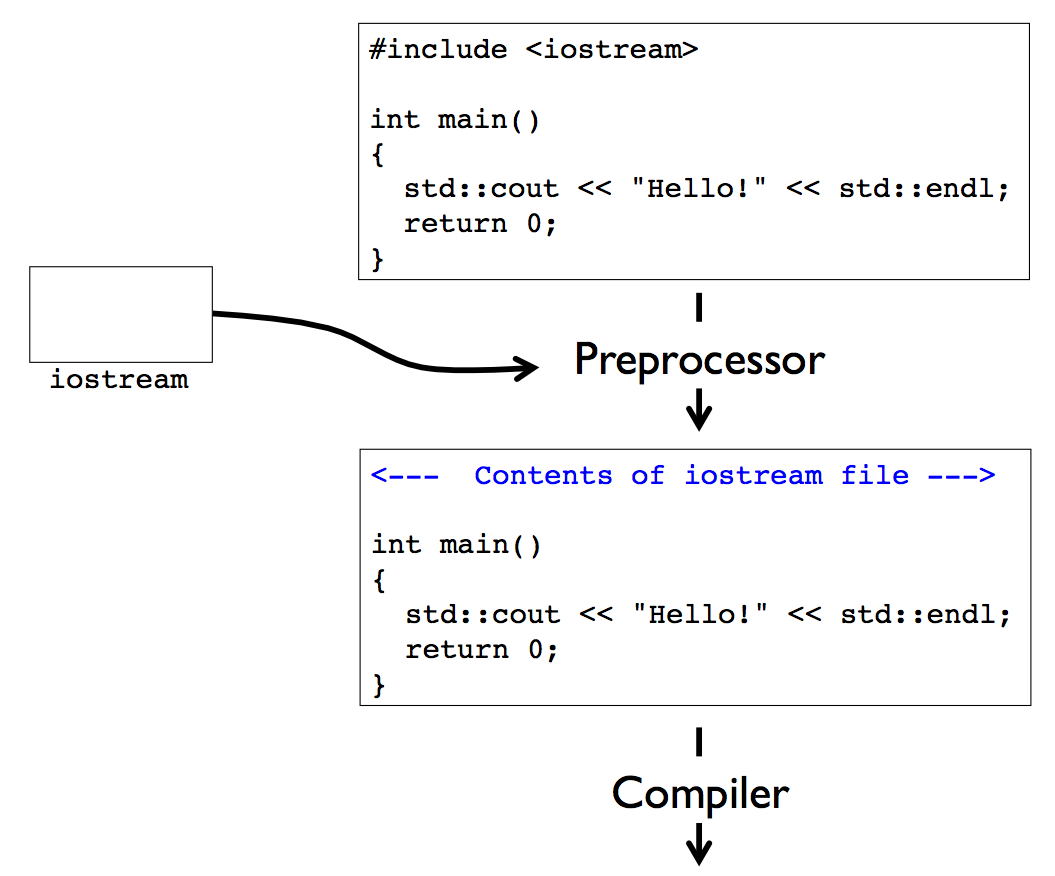
\includegraphics[scale=0.5]{fig/compilation.png}
\caption{\footnotesize When we \texttt{\#include} a library, the contents are effectively inserted
into our source code before compilation continues.}
\end{figure}

\subsubsection{Standard Decomposition of a Program}
\begin{itemize}
\item
  Function (and type) \emph{declarations} go in header (\texttt{.hpp})
  files.
\item
  Function \emph{definitions} go in source (\texttt{.cpp}) files.
\item
  Source files that want to use the functions must \texttt{\#include}
  the header.
\end{itemize}

\texttt{src/main6.cpp}:

\begin{cpp}
#include <iostream> #include "sum6.hpp"
 int main() {
  double a = 2, b = 3;   double c = sum(a,b);
  std::cout << "c = " << c << std::endl;
} \end{cpp}

Then, within \texttt{src/sum6.hpp} we simply include the \emph{prototype} or 
declaration of the function.

\begin{cpp}
double sum(double a, double b);
\end{cpp}

Lastly, within \texttt{src/sum6.cpp} we actually implement the function \emph{definition}.
Realize that we \texttt{\#include} our \texttt{.hpp} file here to ensure it 
gets used in the compilation process.

\begin{cpp}
#include "sum6.hpp"

double sum(double a, double b) {
  double c = a + b;
  return c;
}
\end{cpp}

Now, when we go to compile our \texttt{main} program, we must specify that we have a 
dependency on code contained in \texttt{sum6.cpp}.
Output:

\begin{verbatim}
$ g++ -Wall -Wextra -Wconversion main6.cpp sum6.cpp -o sum6
$ ./sum6
c = 5
\end{verbatim}

\subsubsection{\texttt{\#include} Syntax}
\begin{itemize}
\item
  The \texttt{.hpp} file extension denotes a C++ header file
\item
  \texttt{\textless{}} \texttt{\textgreater{}} around the file name
  means that the preprocessor should search for an include file in a
  system dependent or default directory
\item
  These are typically include files that come with the compiler like
  \texttt{iostream}, \texttt{fstream}, \texttt{string}, etc.
\item
  Usually these files are somewhere in \texttt{/usr/include} with the
  GNU compilers on Linux
\item
  \texttt{"header.hpp"} means that the preprocessor should first search
  in the user directory, followed by a search in a system dependent or
  default directory if necessary
\end{itemize}

\section{\texttt{\#define} and Macros}
\subsection{\texttt{\#define}: A Mini Copy-Paste}
We can use \texttt{\#define} such that anytime the symbol is encountered within our
source code, it gets replaced by a different sequence of characters; e.g.
\texttt{src/define1.cpp}.

\begin{cpp}
// define ni and nj to be 16
#define ni 16
#define nj 16

int main() {
  int a[ni][nj];
  for(int i = 0; i < ni; i++) {
    for(int j = 0; j < nj; j++) {
      a[i][j] = 1;
    }
  }
}
\end{cpp}

Pass the code through the preprocessor, and observe that instances of \texttt{ni} and 
\texttt{nj} have been \emph{replaced} by the value 16, and that comments have been removed!

\begin{verbatim}
$ cpp -P define1.cpp
int main() {
  int a[16][16];
  for(int i = 0; i < 16; i++) {
    for(int j = 0; j < 16; j++) {
      a[i][j] = 1;
    }
  }
}
\end{verbatim}

\subsection{Macros}
The real power of \texttt{\#define} is in setting up macros.
Similar to functions but handled by the preprocessor! They don't involve overhead in
copying arguments into a temporary stackframe which must be set-up and torn-down;
\texttt{src/define2.cpp}.\footnote{Note that
the functionality of Macros for this purpose is largely superceded by compiler optimizations
of inlining functions.}

\begin{cpp}
#include <iostream>

#define sqr(n) (n)*(n)

int main() {
  int a = 2;

  int b = sqr(a);
  std::cout << "b = " << b << std::endl;

  return 0;
}
\end{cpp}

Output:

\begin{verbatim}
$ g++ -Wall -Wextra -Wconversion define2.cpp -o define2
$ ./define2
b = 4
\end{verbatim}

\paragraph{Be Careful: We Really Meant Ctrl-V} The \texttt{\#define} really is a 
copy-paste! I.e. we can omit parentheses at the risk of screwing up our order of operations;
\texttt{src/define3.cpp}.

\begin{cpp}
#include <iostream>

#define sqr(n) n*n

int main() {
  int a = 2;

  int b = sqr(a+3);
  std::cout << "b = " << b << std::endl;
}
\end{cpp}

Output:

\begin{verbatim}
$ g++ -Wall -Wextra -Wconversion define3.cpp -o define3
$ ./define3
b = 11
\end{verbatim}

At this point, you can guess why you can't have an in-line comment following a macro definition!

\subsubsection{Predefined Macros} Several are quite useful, and reminiscent of what we've
encountered in Python;
\texttt{src/define4.cpp}.

\begin{cpp}
#include <iostream>

int main() {
  std::cout << "This line is in file " << __FILE__
            << ", line " << __LINE__ << std::endl;
  return 0;
}
\end{cpp}

Output:

\begin{verbatim}
$ g++ -Wall -Wextra -Wconversion define4.cpp -o define4
$ ./define4
This line is in file define4.cpp, line 5
\end{verbatim}

\subsection{Conditional compilation}
We can use the preprocessor to support conditional compilation using \texttt{ifdef} macros;
\texttt{src/conditional.cpp}.

\begin{cpp}
#include <iostream>

#define na 4

int main() {
  int a[na];

  a[0] = 2;
  for (int n = 1; n < na; n++) a[n] = a[n-1] + 1;

#ifdef DEBUG
  // Only kept by preprocessor if DEBUG defined
  for (int n = 0; n < na; n++) {
    std::cout << "a[" << n << "] = " << a[n] << std::endl;
  }
#endif

  return 0;
}
\end{cpp}

Output:

\begin{verbatim}
$ g++ -Wall -Wextra -Wconversion conditional.cpp -o conditional
$ ./conditional
$ g++ -Wall -Wextra -Wconversion conditional.cpp -o conditional -DDEBUG
$ ./conditional
a[0] = 2
a[1] = 3
a[2] = 4
a[3] = 5
\end{verbatim}

\section{Reading}
\begin{itemize}
\item
  \textbf{C++ Primer, Fifth Edition} by Lippman et al.
\item
  Chapter 6: Functions: Sections 6.1 - 6.3
\item
  Chapter 8: The IO Library
\item
  Chapter 17: Specialized Library Facilities: Section 17.5.1
\item String formatting: \url{http://umich.edu/~eecs381/handouts/formatting.pdf}
\end{itemize}

\end{document}